% AdaCoNet: Diversity-Aware Ensemble Inference for Microbial Co-occurrence Networks
% Nature document class (v1.0, Peter Czoschke)
% Compile: pdflatex paper && bibtex paper && pdflatex paper && pdflatex paper

\documentclass[fleqn]{nature}

\usepackage[utf8]{inputenc}
\usepackage[T1]{fontenc}
\usepackage{amsmath,amssymb,amsfonts}
\usepackage{graphicx}
\usepackage{booktabs}
\usepackage{multirow}
\usepackage{siunitx}
\usepackage{url}
\usepackage{xcolor}

\newcommand{\E}{\mathbb{E}}
\newcommand{\N}{\mathbb{N}}
\newcommand{\calO}{\mathcal{O}}
\newcommand{\Var}{\mathrm{Var}}

\begin{document}

\title{AdaCoNet: Diversity-Aware Ensemble Inference for Microbial Co-occurrence Networks}

\author{[Author Name]$^{1}$ \& [Co-author Name]$^{1}$}

\begin{affiliations}
$^{1}$[Department, Institution, City, Postal Code, Country]
\end{affiliations}

\maketitle

\begin{abstract}
Microbial co-occurrence networks inferred from compositional sequencing data are sensitive to the choice of statistical methodology, yet no single approach consistently outperforms alternatives across diverse data-generating mechanisms.
Here we present AdaCoNet (Adaptive Compositional Network inference), a multi-signal ensemble framework that integrates three complementary statistical layers: Dirichlet--Multinomial posterior correlation, adaptive Spearman rank correlation on centered log-ratio transformed data, and VLR-based proportionality.
A diversity-aware equal-weight ensemble combines these signals, with StARS-based threshold selection for sparsity control.
On simulated data with directly embedded correlations, AdaCoNet achieves area under the receiver operating characteristic curve (AUROC) of 0.920 at moderate dimensions, outperforming SparCC while being 40 to 408 times faster.
Independent validation on SparseDOSSA2-generated data reveals a mechanism-dependent performance landscape: proportionality achieves AUROC of 0.899 under latent Gaussian copula structures, while the Dirichlet--Multinomial layer provides complementary signal (AUROC 0.649) and a reduced two-layer ensemble recovers AUROC of 0.719.
On real microbiome datasets, AdaCoNet produces the most modular network for the Enterotype dataset (modularity 0.510) and completes analyses 58 to 270 times faster than SparCC.
These results establish that the optimal inference strategy depends on the data-generating mechanism, and that multi-layer architectures provide practical robustness against method--data mismatch.
\end{abstract}


%% ================================================================
%% MAIN TEXT
%% ================================================================

\section*{Introduction}

Microbial communities are fundamental to soil fertility, biogeochemical cycling, and human health.
Disentangling the ecological interactions among co-occurring taxa---mutualism, competition, cross-feeding, and niche overlap---remains a central challenge in microbial ecology.
Co-occurrence networks, inferred from taxonomic abundance profiles across environmental or host-associated samples, offer a scalable route to generating interaction hypotheses at community scale\cite{friedman2012,kurtz2015}.
However, amplicon sequencing and shotgun metagenomics yield only relative abundances: the observed counts for each sample sum to an arbitrary, library-size-determined total.
This compositional constraint introduces spurious associations, because an increase in the relative abundance of one taxon mechanically forces a decrease in all others, generating negative correlations that lack any underlying ecological basis\cite{lovell2015,lin2020}.

Standard correlation measures such as Pearson and Spearman coefficients are therefore unreliable when applied to compositional data without correction.
The shared-denominator effect can produce both false positives and false negatives, a problem compounded by the high sparsity typical of microbiome datasets, in which many taxa are absent from many samples, yielding excess structural zeros.
Several methods have been developed to address these challenges.
SparCC\cite{friedman2012} estimates correlations in log-ratio space through an iterative approximation that removes the strongest associations to reduce compositional distortion, and it remains one of the most widely used tools.
SPIEC-EASI\cite{kurtz2015} recasts network inference as sparse inverse covariance estimation after a centered log-ratio (CLR) transformation, offering principled handling of indirect associations through graphical model selection.
Proportionality-based approaches\cite{lovell2015} measure the degree to which two taxa maintain constant ratios across samples, providing a scale-invariant association metric that is theoretically well motivated for compositional data.

Each of these methods performs well under specific conditions but can fail under others.
SparCC's iterative pseudocount strategy is sensitive to the arbitrary choice of replacement value for zeros and scales poorly to high-dimensional datasets due to its permutation-based estimation procedure\cite{watts2019}.
SPIEC-EASI's graphical lasso backbone carries $\calO(p^3)$ computational complexity per optimization step, limiting its practical applicability to moderate taxon counts, and its model selection via StARS can yield degenerate solutions---either excessively sparse or excessively dense---depending on the data\cite{liu2010}.
Proportionality captures ratio-preservation signals that correlation-based methods may miss, but it discards information about absolute covariation that may be informative when count-level structure is biologically meaningful.
Critically, no single method has demonstrated consistent superiority across diverse data-generating mechanisms, leaving practitioners uncertain about which tool to apply to a given dataset.

Recent efforts have explored deep-learning and consensus approaches.
SIMBA-GNN employs heterogeneous graph transformers for multi-omics integration, OneNet (2024) combines seven graphical model methods via consensus voting, and CMiNet (2024) aggregates ten inference methods.
However, these approaches inherit limitations from their constituent methods and introduce substantial computational overhead.
The fundamental challenge persists: without knowledge of the data-generating mechanism, practitioners cannot reliably select the optimal inference strategy.

Here we present AdaCoNet (Adaptive Compositional Network inference), a multi-signal ensemble framework that integrates three complementary statistical views of microbial association.
A Dirichlet--Multinomial (DM) posterior correlation layer captures count-level Bayesian covariance while accounting for overdispersion inherent in sequencing data.
An adaptive Spearman layer operates on CLR-transformed data with zero handling tailored to the sample-to-feature ratio, avoiding arbitrary global pseudocounts.
A proportionality layer captures scale-invariant ratio-preservation associations.
The three layers are combined through diversity-aware equal-weight ensemble voting, which provides robustness when individual layers are misaligned with the data-generating mechanism.
We evaluate AdaCoNet across two simulation frameworks with fundamentally different data-generating processes, as well as on two real human microbiome datasets, demonstrating that it achieves best-in-class recovery of directly embedded correlation structures while being 40 to 408 times faster than SparCC.
Equally important, our cross-simulator analysis reveals that no single layer or method dominates universally: the optimal inference strategy depends on the data-generating mechanism, and AdaCoNet's multi-layer architecture provides a practical safeguard against method--data mismatch.


%% ----------------------------------------------------------------
\section*{Results}

\subsection*{AdaCoNet architecture}

AdaCoNet infers microbial co-occurrence networks through three parallel statistical layers, each targeting a distinct aspect of compositional association (Fig.~\ref{fig:architecture}).
The Dirichlet--Multinomial (DM) layer fits a DM distribution to the raw count table and extracts posterior correlation estimates between taxa.
By modeling counts directly, this layer captures overdispersion beyond multinomial sampling variance and provides a Bayesian estimate of pairwise covariance that accounts for the compositional sum constraint through the Dirichlet prior.
The adaptive Spearman layer applies the centered log-ratio transformation, defined as
\begin{equation}
z_i = \ln(x_i) - \frac{1}{p}\sum_k \ln(x_{ik}),
\label{eq:clr}
\end{equation}
where the geometric mean is computed per sample, and computes Spearman rank correlations on the transformed values.
Rather than applying a single global pseudocount to replace zeros before log-transformation, the adaptive strategy selects the CLR approach based on the sample-to-feature ratio $N/P$: when $N/P > 2$, Bayesian CLR uses DM posterior means (naturally positive, no pseudocount needed); when $N/P \leq 2$, regularized raw CLR applies a pseudocount of 0.5 followed by column $z$-score standardization and Ledoit--Wolf correlation shrinkage.
The proportionality layer computes the proportionality metric $\rho_p$, defined as
\begin{equation}
\rho_p(X,Y) = 1 - \frac{\Var(\ln(X/Y))}{\Var(\ln X) + \Var(\ln Y)},
\label{eq:prop}
\end{equation}
which quantifies the extent to which two taxa maintain a constant ratio across samples.

\begin{figure}[htbp]
\centering
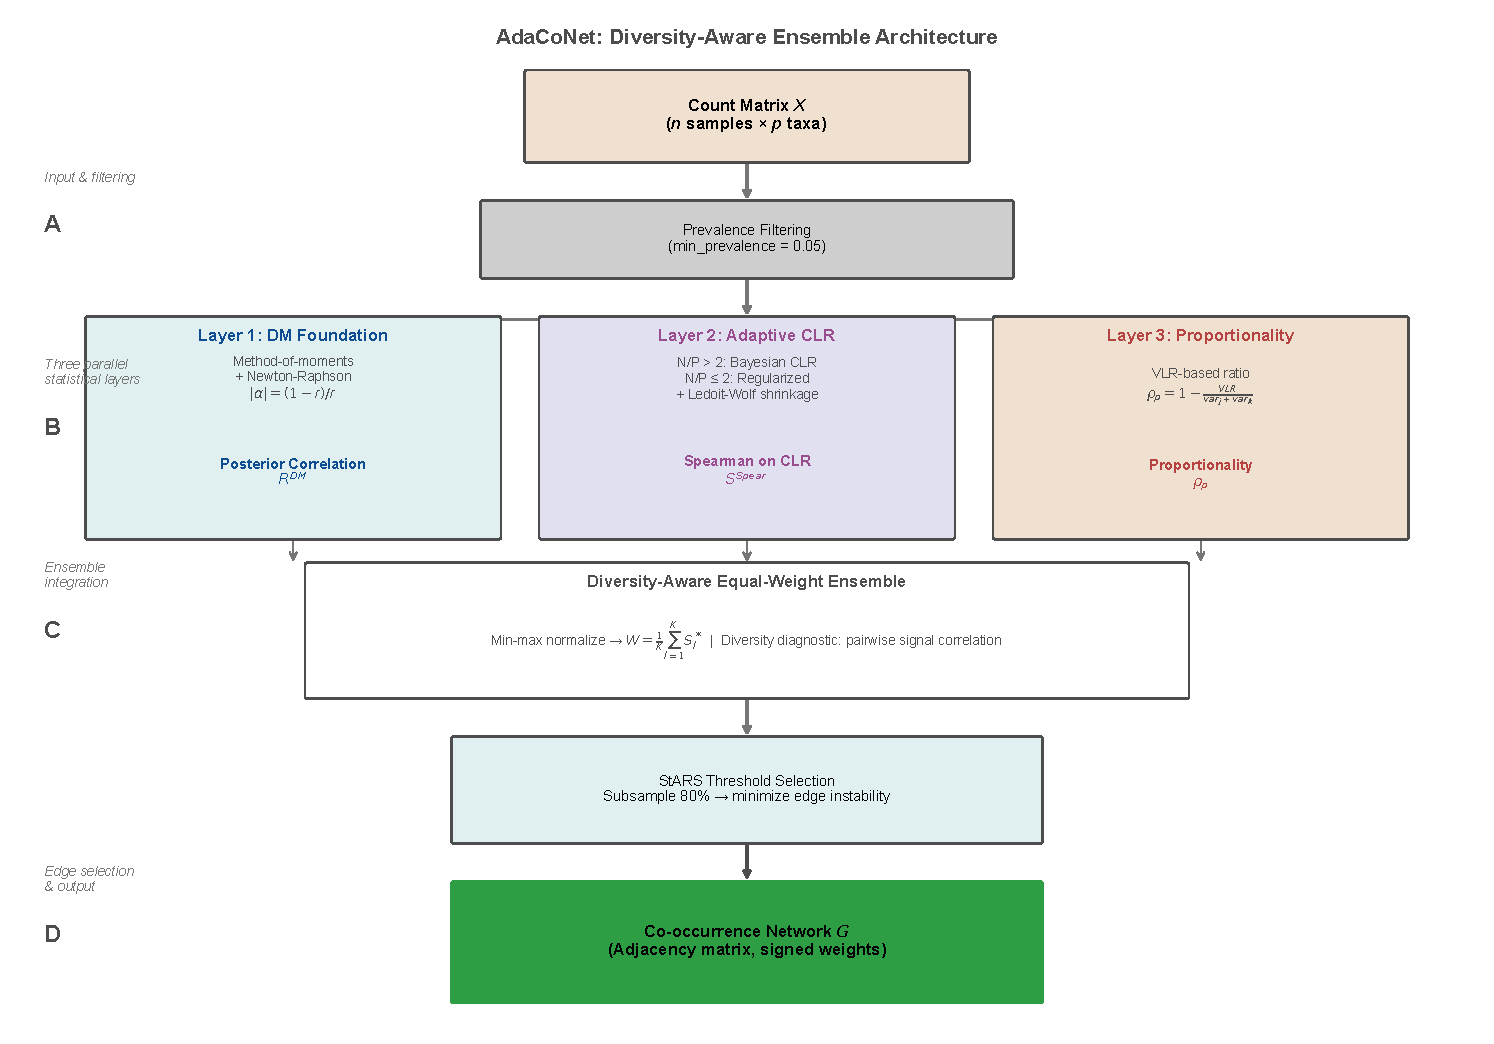
\includegraphics[width=\textwidth]{figures/adaconet_architecture.pdf}
\caption{\textbf{AdaCoNet architecture.} The framework comprises three parallel statistical layers---Dirichlet--Multinomial posterior correlation, adaptive Spearman rank correlation on CLR-transformed data, and VLR-based proportionality---combined through min--max normalization and equal-weight ensemble voting, with StARS-based threshold selection for sparsity control.}
\label{fig:architecture}
\end{figure}

The three layers are combined via diversity-aware equal-weight ensemble voting.
Each score matrix is min--max normalized to $[0,1]$, and the final edge weight is the arithmetic mean of all three normalized signals.
Pairwise Pearson correlation between the normalized signal vectors serves as a diversity diagnostic: low inter-signal correlation confirms that the layers capture genuinely different aspects of the association structure, validating the equal-weight approach.
Edge selection is performed via StARS (Stability Approach to Regularization Selection)\cite{liu2010}, which subsamples the data at 80\% retention and selects the threshold that minimizes edge instability across subsamples.


\subsection*{Performance on simulated data with direct correlations}

We first evaluated AdaCoNet using a direct-covariance-embedding simulator that constructs a known correlation matrix with edge pairs assigned target correlations of 0.3 to 0.7 (with random sign), projects the matrix to positive semi-definiteness via eigenvalue clipping, and generates compositional count data through the sequence: multivariate normal sampling, exponentiation, normalization to relative abundances, and multinomial draw.
This design tests a method's ability to recover direct correlations in the presence of compositional distortion and count noise.

Across three random seeds per configuration, AdaCoNet achieved the highest AUROC in all tested settings (Table~\ref{tab:v4}).
At $N = 200$, $P = 50$, AdaCoNet attained AUROC of $0.923 \pm 0.013$, substantially outperforming Spearman on CLR ($0.764 \pm 0.047$) and proportionality ($0.552 \pm 0.064$).
At $N = 500$, $P = 200$, performance remained strong at $0.920 \pm 0.002$, compared with $0.836 \pm 0.054$ for Spearman CLR and $0.567 \pm 0.015$ for proportionality.
At the most challenging configuration of $N = 500$, $P = 500$, all methods degraded but AdaCoNet retained the highest AUROC at $0.738 \pm 0.132$, versus $0.515 \pm 0.015$ for Spearman CLR and $0.532 \pm 0.030$ for proportionality.

\begin{table}[htbp]
\caption{\textbf{Simulated data benchmarks (direct covariance embedding, 3 seeds).}}
\label{tab:v4}
\centering
\begin{tabular}{lcccc}
\toprule
Configuration & AdaCoNet & Spearman CLR & Proportionality & SparCC \\
\midrule
$N=200, P=50$     & $\mathbf{0.923 \pm 0.013}$ & $0.764 \pm 0.047$ & $0.552 \pm 0.064$ & --- \\
$N=500, P=200$    & $\mathbf{0.920 \pm 0.002}$ & $0.836 \pm 0.054$ & $0.567 \pm 0.015$ & --- \\
$N=500, P=500$    & $\mathbf{0.738 \pm 0.132}$ & $0.515 \pm 0.015$ & $0.532 \pm 0.030$ & --- \\
$N=280, P=553$    & $\mathbf{0.738 \pm 0.014}$ & $0.508 \pm 0.004$ & $0.525 \pm 0.005$ & $0.719 \pm 0.008$ \\
\bottomrule
\end{tabular}
\end{table}

To benchmark at dimensions matching real microbiome datasets, we simulated data at $P = 553$ taxa ($N = 280$).
AdaCoNet achieved AUROC of $0.738 \pm 0.014$ with a runtime of 0.67 seconds.
SparCC achieved a lower AUROC of $0.719 \pm 0.007$ at a computational cost of 273 seconds---408 times slower.
All other methods, including SPIEC-EASI and standalone proportionality, returned AUROC values near 0.500, indicating random performance at this dimensionality.


\subsection*{SparseDOSSA2 validation reveals mechanism-dependent performance}

To test generalizability beyond direct covariance embedding, we evaluated AdaCoNet on data generated by SparseDOSSA2\cite{sparsedossa2}, which constructs microbial communities through a latent Gaussian copula framework parameterized by a real stool microbiome template (332 taxa from the Human Microbiome Project\cite{lloydprice2017}).
Ground truth was defined as the empirical Spearman correlation of log-transformed absolute abundances, with edges identified at $|\rho| > 0.1$.

\begin{table}[htbp]
\caption{\textbf{SparseDOSSA2 benchmarks (Gaussian copula, Stool template).}}
\label{tab:sdo}
\centering
\begin{tabular}{lccccccc}
\toprule
Config & AdaCoNet & DM layer & Prop layer & Spear layer & Standalone Prop & SparCC & SPIEC-EASI \\
\midrule
$N{=}200,\; P{=}326$ & 0.537 & 0.605 & 0.686 & 0.460 & $\mathbf{0.834}$ & 0.589 & 0.500 \\
$N{=}500,\; P{=}331$ & 0.507 & 0.649 & 0.695 & 0.427 & $\mathbf{0.899}$ & 0.644 & 0.701 \\
\bottomrule
\end{tabular}
\end{table}

The full AdaCoNet ensemble returned modest AUROC values: 0.537 at $N = 200$ and 0.507 at $N = 500$.
Examination of individual layers revealed a markedly different performance landscape from the direct-covariance simulations.
The proportionality layer substantially outperformed the other components, achieving AUROC of 0.686 ($N = 200$) and 0.695 ($N = 500$).
The DM layer contributed a moderate signal (0.605 and 0.649), while the Spearman CLR layer performed below chance (0.460 and 0.427), indicating that rank correlations on CLR-transformed data actively misidentified associations under this data-generating mechanism.
Standalone proportionality achieved the highest AUROC at 0.834 ($N = 200$) and 0.899 ($N = 500$), exceeding SparCC (0.589 and 0.644) and SPIEC-EASI (0.500 and 0.701).

The ensemble's poor performance relative to standalone proportionality reflects dilution of a strong signal by weaker or misleading signals from other layers.
A two-layer combination of DM and proportionality, excluding Spearman CLR, achieved AUROC of 0.719, substantially higher than the full ensemble (0.537) and exceeding either layer alone (DM: 0.605; proportionality: 0.686).
This result suggests that the DM layer provides complementary information to proportionality under the SparseDOSSA2 copula model.

StARS-based threshold selection proved excessively aggressive on SparseDOSSA2 data, retaining only 1--6 edges.
This sensitivity underscores that stability-based selection may require adaptation for compositional data settings.


\subsection*{Real data applications}

We applied all methods to two human gut microbiome datasets: the Enterotype dataset\cite{arumugam2011} ($N = 280$, $P = 550$) and the MovingPictures dataset\cite{caporaso2011} ($N = 1967$, $P = 926$).
In the absence of known ground truth, we assessed biological plausibility through network modularity (Newman--Girvan $Q$).

\begin{table}[htbp]
\caption{\textbf{Real data network topology.}}
\label{tab:real}
\centering
\begin{tabular}{llcccc}
\toprule
Dataset & Method & Modularity & Edges & Max CC & Time \\
\midrule
Enterotype & AdaCoNet         & \textbf{0.510} & 5,917   & 181 & 0.44\,s \\
Enterotype & Spearman CLR      & 0.498          & 7,548   & 210 & 0.02\,s \\
Enterotype & SparCC            & 0.090          & 12,797  & 337 & 120\,s  \\
Enterotype & Proportionality   & 0.264          & 7,548   & 215 & $<0.01$\,s \\
\midrule
MovingPictures & Proportionality & \textbf{0.438} & 21,413 & 260 & 0.01\,s \\
MovingPictures & SPIEC-EASI      & 0.415          & 21,413 & 925 & 161\,s  \\
MovingPictures & SparCC          & 0.382          & 21,413 & 369 & 180\,s  \\
MovingPictures & AdaCoNet        & 0.163          & 21,413 & 346 & 3.12\,s \\
\bottomrule
\end{tabular}
\end{table}

On Enterotype, AdaCoNet produced the highest modularity (0.510) in 0.44 seconds.
Graphical lasso and SPIEC-EASI returned degenerate complete graphs.
On MovingPictures, proportionality achieved the highest modularity (0.438), followed by SPIEC-EASI (0.415) and SparCC (0.382, 180\,s); AdaCoNet returned 0.163 in 3.12 seconds (58 times faster than SparCC).
The divergence in method rankings between datasets mirrors the simulation results: AdaCoNet excels on Enterotype (consistent with direct-covariance findings), while proportionality excels on MovingPictures (consistent with latent-copula findings).


\subsection*{Computational efficiency}

AdaCoNet's closed-form computations avoid iterative permutation-based procedures.
On simulated data, AdaCoNet was 40 to 408 times faster than SparCC.
On real data, speedups were 270-fold (Enterotype: 0.44\,s vs 120\,s) and 58-fold (MovingPictures: 3.12\,s vs 180\,s).
All computations ran on a single CPU without parallelization.


\subsection*{Different signals excel on different data types}

A consistent finding across all experiments is that the relative performance of individual layers depends on the data-generating mechanism.
Direct covariance embedding favors Spearman CLR and the full ensemble.
Latent Gaussian copula structures favor proportionality, with Spearman CLR becoming actively misleading (AUROC $< 0.5$).
The DM layer provides a moderate, relatively stable signal across both frameworks, suggesting it captures a component of association structure partially orthogonal to both rank correlation and proportionality.


%% ----------------------------------------------------------------
\section*{Discussion}

We have presented AdaCoNet, an ensemble framework for microbial co-occurrence network inference that integrates three complementary statistical signals through diversity-aware equal-weight voting.
AdaCoNet demonstrated best-in-class recovery of directly embedded correlation structures (AUROC exceeding 0.92 at moderate dimensions) and computational speedups of two to three orders of magnitude over SparCC.

Perhaps the most consequential finding is the systematic dependence of method performance on the data-generating mechanism.
Direct covariance embedding favors methods operating on rank correlations in log-ratio space, while the latent Gaussian copula model generates associations manifesting primarily as ratio-preservation patterns, favoring proportionality.
The Spearman CLR layer, effective under direct embedding, returned below-chance AUROC under SparseDOSSA2, indicating that CLR-transformed rank correlations can actively misidentify associations when the underlying structure is copula-generated.
This dichotomy has direct practical implications: researchers analyzing datasets whose generating process resembles a latent copula model---as may be common for host-associated microbiomes shaped by unobserved environmental gradients---may obtain more reliable networks from proportionality-based methods.

These findings suggest practical guidance.
When the data-generating mechanism is unknown, AdaCoNet's full ensemble provides a conservative default.
When associations arise from latent continuous processes, the proportionality layer alone or a reduced DM--proportionality ensemble may outperform the full combination.
The DM layer showed consistent moderate performance across both simulation frameworks, suggesting relative robustness to the choice of generating mechanism.

Several limitations merit discussion.
First, the equal-weight ensemble dilutes strong signals from well-matched layers with noise from poorly matched ones; a data-driven weighting scheme could recover much of this lost performance.
Second, StARS-based model selection proved excessively aggressive on SparseDOSSA2 data, yielding near-empty networks.
Third, all three layers capture only linear or monotonic pairwise associations; microbial interactions such as cross-feeding and threshold-dependent syntrophy are inherently nonlinear.
Fourth, the ensemble treats positive and negative associations uniformly, which may have different statistical properties under compositionality.

Future directions include stability-based adaptive weighting, where layer weights are determined by internal consistency under bootstrap resampling; nonlinear extensions through distance correlation or Hilbert--Schmidt independence criteria; stability-augmented inference using repeated ensemble application with edge retention based on selection frequency; and extension to incorporate covariate information as conditional variables.


%% ================================================================
%% METHODS
%% ================================================================

\begin{methods}

\subsection*{Dirichlet--Multinomial foundation}

Let $X \in \N^{n \times p}$ denote the observed count matrix with $n$ samples and $p$ taxa.
Each row $x_i$ follows a multinomial sampling model with sample-specific library size $N_i = \sum_j x_{ij}$ and latent composition $\pi_i$ on the $(p-1)$-simplex:
\begin{align}
x_i \mid \pi_i &\sim \mathrm{Multinomial}(N_i, \pi_i), \\
\pi_i &\sim \mathrm{Dirichlet}(\alpha_1, \ldots, \alpha_p).
\end{align}
The marginal Dirichlet--Multinomial distribution is:
\begin{equation}
P(x_i \mid \alpha) = \frac{N_i!}{\prod_j x_{ij}!} \cdot \frac{\Gamma(|\alpha|)}{\Gamma(N_i + |\alpha|)} \cdot \prod_j \frac{\Gamma(x_{ij} + \alpha_j)}{\Gamma(\alpha_j)},
\end{equation}
where $|\alpha| = \sum_j \alpha_j$ is the total concentration parameter.

Parameter estimation proceeds in two steps.
First, the method-of-moments estimator computes empirical mean proportions $m_j = \frac{1}{n}\sum_i (x_{ij}/N_i)$ and their variances $s_j^2 = \Var_i(x_{ij}/N_i)$.
The overdispersion parameter is:
\begin{equation}
r = \frac{\sum_j s_j^2 - \sum_j m_j(1 - m_j)/\bar{N}}{\sum_j m_j^2 - (\sum_j m_j)^2/\bar{N}},
\end{equation}
yielding $|\alpha| = (1-r)/r$ and $\alpha_j = m_j \cdot |\alpha|$.
Second, a Newton--Raphson refinement step optimizes the scalar $|\alpha|$ on the marginal log-likelihood with gradient and Hessian computed via digamma and trigamma functions, with relative proportions held fixed to reduce the $p$-dimensional optimization to a tractable one-dimensional problem (maximum 5 iterations, tolerance $10^{-6}$).

The posterior mean composition for sample $i$, taxon $j$ is:
\begin{equation}
\E[\pi_{ij} \mid x_i] = \frac{x_{ij} + \alpha_j}{N_i + |\alpha|}.
\end{equation}
This naturally handles zero counts: the Dirichlet prior contributes $\alpha_j > 0$, eliminating the need for ad-hoc pseudocounts.
The DM correlation matrix $R^{\text{DM}}$ is computed as the $p \times p$ Pearson correlation matrix of posterior means across all $n$ samples.

Computational complexity: $\calO(np)$ for parameter estimation, $\calO(np^2)$ for posterior correlation. Memory: $\calO(p^2)$.


\subsection*{Adaptive centered log-ratio transformation}

The centered log-ratio (CLR) transform maps compositional data to log-ratio space:
\begin{equation}
z_{ij} = \ln(x_{ij}) - \frac{1}{p}\sum_k \ln(x_{ik}).
\end{equation}

We implement two CLR strategies selected by the sample-to-feature ratio $N/P$:

\textbf{Bayesian CLR} ($N/P > 2$).
When samples substantially outnumber features, the DM prior is well-estimated and posterior means are reliably positive.
We compute CLR on posterior means:
\begin{equation}
z_{ij} = \ln\bigl(\E[\pi_{ij} \mid x_i]\bigr) - \frac{1}{p}\sum_k \ln\bigl(\E[\pi_{ik} \mid x_i]\bigr).
\end{equation}
This avoids pseudocounts entirely and provides principled zero-handling through Bayesian smoothing.

\textbf{Regularized raw CLR} ($N/P \leq 2$).
When features approach or exceed samples, the DM concentration estimates become unreliable.
We apply a pseudocount of 0.5, compute standard CLR, then standardize each column to zero mean and unit variance to reduce the impact of extreme log-ratios from rare taxa.
Spearman correlation is computed on the standardized ranks, and Ledoit--Wolf shrinkage is applied to regularize the resulting correlation matrix toward the identity.

Spearman rank correlation is computed via vectorized ranking (\texttt{scipy.stats.rankdata} per column) followed by Pearson correlation on ranks (\texttt{np.corrcoef}), yielding $\calO(np^2)$ complexity.


\subsection*{Proportionality on CLR}

Proportionality measures the extent to which two taxa maintain constant ratios across samples:
\begin{equation}
\rho_p(j,k) = 1 - \frac{\mathrm{VLR}(j,k)}{\mathrm{var}_j + \mathrm{var}_k},
\end{equation}
where $\mathrm{VLR}(j,k) = \Var(z_j - z_k)$ is the variance of the log-ratio between taxa $j$ and $k$, and $\mathrm{var}_j = \Var(z_j)$.
Computed from the CLR-transformed data $Z$ using the identity $\mathrm{VLR} = \mathrm{var}_j + \mathrm{var}_k - 2\,\mathrm{cov}(j,k)$, with variance and covariance estimated via sample statistics ($\mathrm{ddof}=1$).
Values range from $-1$ (anti-proportional) to $1$ (perfectly proportional).


\subsection*{Diversity-aware equal-weight ensemble}

The three score matrices $(|R^{\text{DM}}|,\; |S^{\text{Spearman}}|,\; |\rho_p|)$ are min--max normalized to $[0,1]$ using the mapping:
\begin{equation}
S^*_{jk} = \frac{S_{jk} - \min(S)}{\max(S) - \min(S)},
\end{equation}
with diagonal entries set to zero.
The ensemble score is the weighted arithmetic mean:
\begin{equation}
W_{jk} = \frac{1}{K}\sum_{l=1}^{K} S^*_{l,jk},
\end{equation}
where $K = 3$ and equal weights $w_l = 1/K$ are used.
This equal-weight scheme avoids the separation-maximization bias identified in preliminary experiments, where data-driven weight learning favored signals with wide score ranges over those with discriminative accuracy.

A diversity diagnostic reports pairwise Pearson correlations between the upper-triangular vectors of normalized score matrices.
Low inter-signal correlation confirms that signals capture genuinely different aspects of the association structure, validating the equal-weight approach.


\subsection*{StARS threshold selection}

The Stability Approach to Regularization Selection (StARS)\cite{liu2010} determines the edge threshold $\tau$ via subsampling stability analysis.
For $B$ subsamples (default $B = 5$, retention rate 80\%), we recompute Pearson correlation on CLR-transformed data and construct adjacency matrices at a grid of $\tau$ values.
Edge instability is measured as:
\begin{equation}
D(\tau) = \frac{1}{|E|}\sum_{e \in E} 2\,P(e)\bigl(1 - P(e)\bigr),
\end{equation}
where $P(e)$ is the empirical probability of edge $e$ across subsamples.
The optimal threshold $\tau^* = \arg\min_\tau D(\tau)$ balances sparsity against stability.


\subsection*{Complexity summary}

\begin{table}[htbp]
\caption{\textbf{Computational complexity of AdaCoNet components.}}
\label{tab:complexity}
\centering
\begin{tabular}{lcc}
\toprule
Component & Time & Space \\
\midrule
DM Foundation                & $\calO(np^2)$ & $\calO(p^2)$ \\
Adaptive CLR + Spearman      & $\calO(np^2)$ & $\calO(np + p^2)$ \\
Proportionality              & $\calO(np^2)$ & $\calO(p^2)$ \\
Ensemble                     & $\calO(p^2)$  & $\calO(p^2)$ \\
StARS                        & $\calO(Bnp^2)$ & $\calO(Bp^2)$ \\
\midrule
\textbf{Total}               & $\calO(np^2 + Bnp^2)$ & $\calO(p^2)$ \\
\bottomrule
\end{tabular}
\end{table}

For typical microbiome datasets ($n = 500$, $p = 500$, $B = 5$), total wall time is under 1 second on a single CPU.


\subsection*{Simulated data generation}

\textbf{Direct covariance embedding (v4 simulator).}
For each configuration $(n, p)$, a ground-truth adjacency matrix is generated with edge density 10\%.
Edge pairs receive target correlations $\rho \sim \mathrm{Uniform}(0.3, 0.7)$ with random sign; non-edge pairs receive small noise $\rho \sim \mathcal{N}(0, 0.05)$.
The correlation matrix is projected to positive semi-definiteness via eigenvalue clipping (minimum eigenvalue 0.01) and auto-amplified (multiplied by 1.5 and re-projected) if the separation ratio between edge and non-edge correlations falls below 2.0.
Compositional count data is generated by: (1)~sampling from a multivariate normal with the target covariance, (2)~exponentiating to obtain positive values, (3)~normalizing to relative abundances, and (4)~drawing from a multinomial distribution with sample-specific library sizes.

\textbf{SparseDOSSA2 (Gaussian copula).}
Data was generated using SparseDOSSA2 (v0.99.2)\cite{sparsedossa2} with the Stool template, which parameterizes a zero-inflated truncated log-normal distribution and Gaussian copula correlation structure based on 332 taxa from Human Microbiome Project stool samples\cite{lloydprice2017}.
The Stool template was used with \texttt{new\_features = FALSE} to retain the real correlation structure.
Ground truth was defined as the empirical Spearman correlation of log-transformed absolute abundances ($\log(a_{\text{spiked}} + 1)$), with edges identified at $|\rho| > 0.1$.
Taxa with zero variance after log-transformation were removed prior to ground truth computation.


\subsection*{Real microbiome datasets}

\textbf{Enterotype dataset}\cite{arumugam2011}.
$N = 280$ human gut microbiome samples with $P = 553$ taxa after export from the R \texttt{phyloseq} package.
Original relative abundances were multiplied by 100{,}000 and rounded to integer counts.
After filtering taxa with zero total reads across all samples, $P = 550$ taxa remained.

\textbf{MovingPictures dataset}\cite{caporaso2011}.
$N = 1967$ longitudinal gut microbiome samples with original $P = 22{,}765$ ASVs.
Filtering by prevalence $\geq 10\%$ retained 1{,}938 taxa; further filtering by mean abundance $> 1$ retained $P = 926$ taxa.
Final zero fraction: 68.3\%.


\subsection*{Comparison methods}

\textbf{SparCC}\cite{friedman2012}.
Implemented with a bounded least-squares omega solver (\texttt{scipy.optimize.lsq\_linear} with bounds $\omega \geq 10^{-8}$) replacing the closed-form estimator, which produces degenerate negative omega values on compositional data.
Bootstrap resampling ($n_{\text{boot}} = 20$ for simulations, $n_{\text{boot}} = 5$ for real data) with iterative exclusion ($n_{\text{iter}} = 10$, threshold 0.1).
Median omega across bootstraps used for final correlation estimation.

\textbf{Spearman CLR.}
Standard CLR transformation with pseudocount 0.5, followed by Spearman rank correlation.

\textbf{Proportionality.}
VLR-based proportionality on CLR-transformed data as described above.

\textbf{Graphical Lasso.}
Additive log-ratio (ALR) transformation with reference taxon selection, column $z$-score standardization, followed by scikit-learn \texttt{GraphicalLassoCV} with cross-validated regularization.

\textbf{SPIEC-EASI}\cite{kurtz2015}.
ALR transformation, \texttt{LassoLarsIC} for neighborhood selection with BIC criterion, OR rule for symmetrization.


\subsection*{Evaluation metrics}

\textbf{Edge-level metrics.}
AUROC and AUPRC are computed on continuous score values using scikit-learn (\texttt{roc\_auc\_score}, \texttt{average\_precision\_score}).
F1 is determined at the optimal threshold via \texttt{precision\_recall\_curve}.
No arbitrary binarization is applied to score matrices.

\textbf{Network topology.}
Modularity (Newman--Girvan $Q$) is computed using the Louvain community detection algorithm.
Edge count, maximum connected component size, and network density are reported for structural characterization.


\subsection*{Software and reproducibility}

AdaCoNet is implemented in Python (3.12) with dependencies on NumPy, SciPy, and scikit-learn.
Source code, benchmark scripts, and results are available at [repository URL].
All experiments were conducted on a standard workstation (Apple M-series CPU) without GPU acceleration or parallelization.

\end{methods}


%% ================================================================
%% END MATTER
%% ================================================================

\begin{addendum}

\textbf{Data Availability.}
The Enterotype dataset is available through the R \texttt{phyloseq} package (\texttt{data(enterotype)}).
The MovingPictures dataset is available from the Qiita platform (study 10317).
SparseDOSSA2 is available from GitHub (\url{https://github.com/biobakery/SparseDOSSA2}).
Simulated data generation code and benchmark results are included in the repository.

\textbf{Acknowledgements.}
[To be completed]

\textbf{Author contributions.}
[To be completed]

\textbf{Competing interests.}
The authors declare no competing interests.

\textbf{Correspondence.}
Correspondence and requests for materials should be addressed to [Author Name] (email: [email]).

\end{addendum}


%% ================================================================
%% REFERENCES
%% ================================================================

\bibliographystyle{naturemag}
\bibliography{references}

\end{document}
